\documentclass[12pt]{article}
\usepackage{amssymb,amsmath,times}
\usepackage{color}
\usepackage{graphicx}
\usepackage{fancyhdr}
\usepackage{multirow}
\usepackage{cite}
\usepackage{color}
\usepackage{natbib}

% define formatting
%\pagestyle{empty}
\parindent=0pt
\topmargin=0.in \headheight=0in \headsep=-0.1in \textheight=9.2in
\textwidth=6.5in \oddsidemargin=0in

\def\Neff{{N_{\rm eff}}}
\input{probe_defs.tex}

\setlength{\floatsep}{0.5\floatsep}
\setlength{\textfloatsep}{0.5\textfloatsep}
\setlength{\intextsep}{0.5\intextsep}
\setlength{\floatsep}{0.5\floatsep}
\setlength{\dblfloatsep}{0.5\dblfloatsep}
\setlength{\dbltextfloatsep}{0.5\dbltextfloatsep}

\begin{document}

\bibliographystyle{unsrt}

\setlength{\baselineskip}{1.0\baselineskip}
\setlength{\parskip}{1.\parskip}

\parindent = 15pt

\tableofcontents

\setcounter{figure}{0}

\newpage
%\twocolumn

\section{Scientific, Technical, and Management Section}



\vspace{-0.13in}

\comred{0.5 pg. executive summary goes here: the sky is sunny}
% Shaul


\vspace{-0.22in}


\subsection{Science Objectives}
\label{sec:science}

\vspace{-0.05in}

\comred{5 pages for all science goals including the (temporary) two sections below.}

\subsubsection{The Inflationary Gravitional Wave Background}

\vspace{-0.05in}

\comred{The verbiage below is taken from another proposal. Here we need to explain what are the science objectives 
of the CMBProbe, how the science objectives relate to the current state of knowledge, and to NASA's goals}
% Lloyd, Sarah, Dan, Rafael

The paradigm of inflation~\cite{guth81,linde82,albrecht82,sato81,kolb94}
%, in which the Universe underwent exponential expansion within the first $\sim$$10^{-35}$~sec, 
makes several predictions that are consistent with all current astrophysical 
measurements~\cite{spergel06,Tegmark:2006az,planck2015parameters,planck2015inflation}. 
A robust prediction of inflation is the existence of a stochastic background of gravitational radiation 
with an amplitude depending on the mechanism driving the accelerated 
expansion~\cite{starobinsky82,starobinsky83a,rubakov82,grishchuk75,abbott84a}.
In most scenarios, this `inflationary gravitional wave background' (\igb) is predicted
to have a spatial power spectrum whose amplitude is proportional to the energy
scale of inflation $V^{1/4}$ via
$V^{1/4} = 3.7 \times 10^{16} \ r^{1/4}\,\, {\rm GeV},$
where $V$ is the inflaton potential and $r$ is the ratio of the temperature
quadrupoles produced by gravitional waves and by density perturbations.  
There are theoretical reasons $V^{1/4}$ may be close to the Grand
Unification scale of $10^{16}$~GeV, suggesting detectable $r$ values between 
$\sim$0.001 and $\sim$0.1. In addition to determining the energy scale of inflation, measurements 
of the \igb\ probe the scalar field potential at or above the Planck scale, which is particularly relevant for inflation models motivated 
by string theory~\cite{SnowmassInflationTheory}. Measurements of the \igb\ thus probe fundamental physics at the 
highest possible energy scales. 
\begin{figure}[htbp!]
\hspace{0.in}
\parbox{4.2in}{ \centerline {
\includegraphics[width=2.0in] {Figures/sunny_skies.jpg}  
\hspace{0.1in}
\includegraphics[width=2.0in] {Figures/sunny_skies2.jpg}  }  }
\hspace{0.1in}
\parbox{2.in}{
\caption{ \small \setlength{\baselineskip}{0.90\baselineskip}
       Sample Figure of Sunny Skies
\label{fig:sunny_skies} } }   
\vspace{-0.05in}
\end{figure}

The most promising way to search for the \igb\ is through its signature on the CMB polarization~\cite{kamionkowski97b,seljak97}.  
Primordial energy density perturbations produce only a curl-free, or `E-mode', pattern of polarization.
Gravitional waves also produce a curl, or `B-mode', pattern of polarization that density perturbations cannot
produce~\cite{kamionkowski97a,zaldarriaga97}.  The amplitude of the B mode is related to the energy scale
of inflation by $V^{1/4}=2\times10^{16} \ ( B_{peak} / 0.1\,\mu{\rm
K})^{1/2} \,{\rm GeV},$ where $B_{peak}$ is the amplitude of the power spectrum of the B mode in \microk\ at $\ell=80$;
see Fig.~\ref{fig:sunny_skies}. In its recent report New Worlds New Horizons (NWNH), the decadal survey 
committee strongly endorsed sub-orbital searches for the B-mode signal from 
inflation saying that ``The convincing detection of B-mode polarization in the CMB produced in the 
epoch of reionization would represent a watershed discovery.''~\cite{blandford2010}

B-mode signatures near the expected \igb\ peak at $\ell=80$ have recently been detected by BICEP2~\cite{bicep2Bmode}. 
However, the combination of Planck data with those from the BICEP2 and Keck Array collaborations have demonstrated 
that the B-mode signal measured is entirely consistent with contributions from polarized emission of Galactic dust and the 
signal from the gravitational lensing of CMB photons by the large scale structure of the Universe (see 
Section~\ref{sec:lensing})~\cite{bkp2015,planck2014-XXX,2016PhRvL.116c1302B}. 
These data give an upper limit of $r<0.09$ at 95\% confidence level.
Most importantly, the constraint is largely limited by Planck's noisy measurement of the dust properties in the 353~GHz band; 
a noiseless dust map could shrink the constraint by a factor of two~\cite{bkp2015}. 
Further progress --- detections or improved limits --- requires instruments 
with higher sensitivity at {\it both} the dust and CMB frequency bands so that this Galactic foreground can be properly identified 
and removed. 

\vspace{-0.15in}

\subsubsection{Neutrinos and Light Relics}

\vspace{-0.05in}

Much of the information about our thermal history and the particle content of the universe is encoded in the $T$ and $E$ power spectra.  
A high-precision measurement of these spectra over the full sky is expected to significantly improve our understanding of the post-inflationary 
universe.  This is particularly true in $E$-mode polarization where, to date, far fewer modes have be measured at the level of cosmic variance than in temperature.

The spectra at high-$\ell$ contain important information about the components of the thermal plasma and their interactions around the time of recombination.  One particular compelling target is the effective number of neutrino species, $\Neff$, which parameterizes the total amount of energy density in radiation at the time of recombination.  It is defined such that in the Standard model of particle physics with normal thermal evolution, $\Neff = 3.046$ due to the energy density in the three species of neutrinos.  $\Neff$ is also sensitive to any additional light relic particles as their gravitational influence is identical to the neutrinos.  In fact, if there was an additional light particle in thermal equilibrium with the Standard model particles at any point in our history, it will contribute a change to $\Neff$ of at least $\Delta \Neff \geq g \, 0.027$ where $g \leq 1$ is the number of degrees of freedom of the new particle.  This defines a compelling target of $\sigma(\Neff) < 0.027$ for future CMB observations.  New light particles are a common feature of many approaches to beyond the Standard model physics and can be directly tied to some of the most significant problems in the Standard model.  Either a limit or detection of $\Delta \Neff$ at this level would provide a powerful insight into the laws of nature and our thermal history. 

The presence of free-streaming radiation changes the detailed features of the $TT$, $TE$ and $EE$ spectra at all $\ell$.  In particular, it changes the locations of the acoustic peaks and alters the damping tail at high-$\ell$.  Similar changes to the spectra arise from many other compelling targets including the helium fraction $Y_p$ and more general dark sector physics.  For this reason, constraints on $\Neff$ a useful proxy for the information available in the high-$\ell$ power spectra.  

Preliminary forecasts for $\Neff$ are shown in the right hand panel of Figure~\ref{fig:Neff_future}.  A space-based mission reaching an effective temperature noise of 1-2 $\mu$K-arcmin over the full sky gives competitive constraining power when compared other proposals.  The two most important quantities for improving constraints on $\Neff$ and other high-$\ell$ targets are $f_{\rm sky}$ and the temperature noise.  The full-sky nature of the proposed mission would allow for cosmic variance limited $E$-modes over most of the sky and a large range of $\ell$.

The main downside of a space-based mission is that we cannot reach the resolutions available from the ground.  However, we see that at 5' resolution and 1 $\mu$K-arcminute noise the forecasts are less sensitive to the resolution then one might naively expected.  In particular we can reach $\sigma(\Neff) < 0.035$ for temperature noise from 1-2 $\mu$K-arcmin and $f_{\rm sky} =0.6-0.8$.  These forecasts are competitive with CMB Stage IV.  Specifically, the larger sky fraction and sensitivity available from space appears to compensate for the reduced resolution.  In fact, the full sky measurement would provide complimentary information that could be combined with ground based surveys to further improve over the limits available from either experiment.  This is particularly important for $\Neff$ which is tantalizingly close to the target of $\sigma(\Neff) =0.027$ and therefore even an apparently modest improvement could have a major scientific impact.  

The sum of neutrino masses, $\sum m_\nu$, is another theoretically compelling target that is accessible from Cosmology.  The most distinctive feature of $\sum m_\nu$ is that it suppresses the growth of structure on small scales.  This suppressed can be measure in the CMB through amplitude of the lensing power spectra compared to the primary CMB.  In principle, this relative difference can yield a measurement  of the minimum value of $\sum m_\nu =58$ meV at 4-5 $\sigma$ for a number of future cosmological surveys.  However, sensitivity to $\sum m_\nu$ is ultimately limited by our knowledge of the primordial amplitude of fluctuations $A_s$ which is strongly degenerate with the optical depth $\tau$. 

The current limit on $\tau$ from the Planck satellite of $\tau = 0.055 \pm 0.009$ ultimately limits $\sigma(\sum m_\nu) \gtrsim 25$ meV, as shown in the panel of Figure~\ref{fig:Neff_future}.  While the figure shows the sensitivity of a space-based CMB mission to $\sum m_\nu$, this lower limit is common to any measurement that depends on the relative suppression.  Therefore, a cosmological detection of $\sum m_\nu = 58$ meV at 3-5 $\sigma$ depends crucially on an improvement measurement of $\tau$.  To date, the only proven method for such a measurement is from a space-based CMB observations.  The best constraints on $\tau$ come from $E$-modes with $\ell < 20$ which requires control over the largest angular scales.  


\begin{figure}[t!]
\begin{center}
\includegraphics[width=0.45\textwidth]{figs/Mnu_tauprior.pdf}
\includegraphics[width=0.45\textwidth]{figs/Neff.pdf}
\caption{ {\it Left:} Neutrino mass constraints as a function of the prior on $\tau$ for a 5' beam and sky fraction of $f_{\rm sky} = 0.7$.  The blue dashed line is the Planck blue book expectation and the white dashed line a cosmic variance limit measurement of $\tau$ form the CMB. {\it Right:} $\Neff$ Forecasts as a function temperature noise and sky fraction assuming 5' resolution.}
\label{fig:Neff_future}
\end{center}
\end{figure}



\vspace{-0.15in}
\subsubsection{CMB spectral distortion science}
\vspace{-0.05in}

In addition to the CMB temperature and polarization anisotropies targeted by CMB imagers, {\it unique} new information about early-universe physics can be gained by studying the energy spectrum of the CMB \citep{Sunyaev1970SPEC, Burigana1993, Hu1993, Chluba2011therm}. The measurements of COBE/FIRAS have shown that the average CMB spectrum is extremely close to that of a blackbody at a temperature $T_0=(2.726\pm 0.001)\,{\rm K}$ \citep{Mather1994, Fixsen1996}. However, several standard processes are expected to {\it distort} the CMB spectrum \citep[e.g.,][]{Chluba2016LCDM} at a level that is within reach of present-day technology \citep{Kogut2011PIXIE, PRISM2013WPII}. 
%
The classical distortion shapes are known as Compton-$y$ and chemical potential ($\mu$-type) distortions \citep{Zeldovich1969, Sunyaev1970mu} and are caused by energy exchange of CMB photons with free electrons. A $\mu$-distortion can only be produced in a hot and dense environment present at redshifts $z\gtrsim 5\times10^4$, while $y$-type distortions appear at lower redshifts. This makes $\mu$-distortions a unique messenger from the early Universe.

The largest guaranteed distortion is caused by the late-time energy release of forming structures and from reionization \citep{Sunyaev1972b, Hu1994pert, Oh2003, Cen1999, Refregier2000}, imprinting a $y$-type distortion with $y \simeq 2\times 10^{-6}$ \citep[e.g.,][]{Refregier2000, Hill2015}. This distortion is only one order of magnitude below the current limit from COBE/FIRAS and, even with most pessimistic assumptions about foregrounds, should be clearly seen with next-generation spectrometers, telling us about the total energy output of first stars, AGN and galaxy clusters. In particular, group-size clusters ($M\simeq 10^{13}\,M_{\odot}$) contribute significantly to the signal. These are still sufficiently hot (temperature $k T_{\rm e}\simeq 1\,{\rm keV}$) to create a visible relativistic temperature correction to this large $y$-distortion, which could be used to constrain cluster feedback models \citep{Hill2015}. These two inevitable signals probe the low-redshift Universe and provide clear targets for future spectral distortions measurements and their requirements in the presence of foregrounds.

Next generation CMB spectrometers are also expected to greatly improve the $\mu$-distortion limits of COBE/FIRAS \citep{Kogut2011PIXIE}. This will allow us to place stringent bounds on the presence of long-lived decaying particles \citep{Hu1993b, Chluba2013fore, Chluba2013PCA, Dimastrogiovanni2015} and other new physics \citep[e.g.,][]{Jedamzik2000, Tashiro2012, Dolgov2013, Tashiro2013, Caldwell2013, Yacine2015DM}, but a clear target is predicted by the dissipation of small-scale perturbation through Silk-damping \citep{Sunyaev1970diss, Daly1991, Hu1994, Chluba2012}. This process allows us to place stringent constraints on the amplitude of the small-scale curvature power spectrum, present at scales (wavelength $0.1 \,{\rm kpc} \lesssim \lambda \lesssim 1\, {\rm Mpc}$) and epochs ($10^4 \lesssim z\lesssim 10^6$) inaccessible through any other observation. This delivers a complementary test for the inflation paradigm \citep{Chluba2012inflaton, Dent2012, Chluba2013PCA, Clesse2014, Cabass2016}, with $\mu=(2.0\pm0.14)\times 10^{-8}$ expected in $\Lambda$CDM \citep{Chluba2016LCDM}. Precise measurements of signals at this level will be extremely challenging and requires unprecedented control of systematics and modeling of foregrounds. It would also bring us to the sensitivity level required to detect the cosmological recombination radiation \citep{Sunyaev2009, Chluba2016} imprinted by the recombination of hydrogen and helium at redshift $z\simeq 10^3-10^4$. Optimizing next-generation CMB spectrometers for these purposes requires extensive studies.

Aside from the average CMB distortion signals, the CMB spectrum can also vary across the sky. One source of anisotropic distortions is related to clusters of galaxies and has already been measured \citep{Planck2013SZ}. A combination of precise CMB imaging and spectroscopic measurements might allow observing the relativistic temperature correction  \citep{Sazonov1998, Itoh98, Challinor98} of individual SZ clusters. This could allow us to calibrate cluster scaling relations and learn about the dynamical state of the cluster atmosphere. Anisotropies in the $\mu$-distortion can be created through ultra-squeezed limit non-Gaussianity \citep{Pajer2012, Ganc2012} and could be used to probe scale-dependent non-Gaussianity \citep{Biagetti2013, Razi2015}. Finally, resonant scattering signals in the recombination \citep{Jose2005, Carlos2007Pol, Lewis2013} and post-recombination eras \citep{Kaustuv2004, Schleicher2008} can lead to spectral-spatial CMB signals that can be used to constrain the presence of metals in the dark ages and the physics of recombination. For all these applications, instrumental synergies between CMB imaging and spectroscopy need to be studied in detail. 


In summary, future studies of the CMB spectrum will open a new {\it unexplored} window to early phases of the Universe ($z > 10^3$), which cannot be probed in any other way. This will not only allow us to test the standard cosmological paradigm (e.g., inflation and reionization) but also opens up a huge discovery space to non-standard physics (e.g., decaying/annihilating particles). This immense potential and complementarity with CMB anisotropy studies makes CMB spectral distortions an important future target and identifying experimental routes towards extracting these tiny signals from the early Universe will be one main objective of the proposed mission study.

\vspace{-0.15in}
\subsubsection{The Cosmic Infrared Background} 
\vspace{-0.05in}
A significant foreground contamination for CMB studies at
intermediate and small scales is due to the extragalactic
emission from infrared (IR) sources responsible for the Cosmic
Infrared background (CIB). The CIB is the second largest
extragalactic background after the CMB, with an approximate
brightness of 24 W m$\mathrm{^-2 sr^-1}$ (Dole).\\
Dust enshrouding star-forming galaxies is heated by starlight
at ultraviolet (UV) and optical wavelengths, and re-radiates at
mid-IR to sub-millimetre wavelengths. Thus, the integrated emission
from galaxies actively producing stars at the peak of star formation
($\mathrm{z\sim 1-3}$) reaches us in the far-infrared (FIR) regime,
carrying a wealth of information about the history of star formation,
dust production, and the growth of large-scale structures.
The drawback of working with a high density of faint, distant sources in the FIR
regime is that individual objects are blended. For {\it Herschel}
maps, only 10$\%$ of the objects has been resolved
into individual galaxies at 857 GHz, and less than 1$\%$ at 600 GHz
\cite{bethermin2012}. However, the anisotropies detected in the
unresolved background trace the clustering of star-forming galaxies,
and the distribution of the underlying dark matter field.
Similarly to the CMB, they can be studied through statistical tools
such as the angular power spectrum \citep{knox2001}, and interpreted with current
phenomenological models linking dark halos to galaxies, such as the Halo model \cite{shang}.
Recently, two major ESA/NASA satellites, {\it Herschel} and {\it Planck},
performed ground-breaking measurements of the CIB,
allowing us to gain new insights on the star formation
history of the Universe and the link between CIB sources
and the dark matter. There are many reasons to go further,
and measure CIB anisotropies with increasing sensitivity at both large and small scales.
\begin{itemize}
\item The CIB is a full sky, bright, high redshift extragalactic
background that maps star formation at its peak. While the
CIB is not our only handle on the cosmic star formation rate (SFR),
it is particularly important because FIR/sub-millimetre surveys do
not suffer from a number of uncertain steps in the conversion from
galaxy counts and luminosities to star formation rates, affecting, e.g., optical surveys.
The Planck Collaboration, analyzing CIB anisotropies and their correlation with CMB lensing,
recently derived constraints on the star formation rate density which, at redshift $z>2$, are higher
than what expected from other analyses \cite{madau2014}.
Future measurements of CIB power spectra will shed light on this important issue.
\item The CIB is a tracer of the dark matter field with a broad redshift kernel, and it can be
used in cross-correlation with many other datasets to explore the link between light and matter.
The cross-correlation with the CMB lensing and with LSS galaxies has been explored by **** and
they allows us to constrain the bias between CIB sources and the dark matter,
and the redshift distribution of the galaxies making up the CIB, complementing the information coming
from CIB anisotropies alone. Many other possible cross-correlations are being explored. Recently
Cooray...
\item The CIB is an important foreground for CMB studies. As shown in
Planck Collaboration (Likelihood), a significant contribution to the
astrophysical foreground in the 143x217 and 217x217 GHz channels at
intermediate and small scales in due to the clustering and Poisson
components of the CIB. The cross-correlation between infrared galaxies and the thermal
Sunyaev-Zeldovich (tSZ) effect provides an additional contamination. An accurate
determination of the CIB auto-power spectra and CIB-tSZ power spectra will be fundamental to
reduce the uncertainties in the CMB parameter estimation
\item Delensing of the CMB: The CIB, being a tracer of the dark matter field in a broad redshift range,
is heavily correlated with the lensing convergence. Recent efforts by Sherwin and Schmittfull and
Larsen et al. have shown that the combination of Planck CIB maps at 545 and 857 GHz can be used as a
lensing tracer to reverse the lensing distortion on Planck CMB temperature maps. Upcoming CMB surveys
will heavily rely on delensing methods for investigating the small inflationary B-mode polarization signal,
and accurate CIB templates will be crucial for this task.
\end{itemize}
The new mission probe, following Planck’s steps, will measure CIB anisotropies at large and
intermediate scales, and in multiple frequency channels.
With only one tenth of {\it Planck}'s instrumental noise,
the small-scale power spectrum will be measured with unprecedented
precision, in the critical range where the clustering due to galaxies
in the same dark matter halo is similar in amplitude to the clustering
due to galaxies in separated halos (2-halo term).



\vspace{-0.22in}

\subsection{The Challenges: Foregrounds, systematics}
\label{sec:foregrounds}
\vspace{-0.05in}
\comred{3 pages. Discuss the challenge of Foregrounds and Systematics. }

\begin{figure}[h]
\begin{center}
\includegraphics[width=3.2in]{Figures/P15_2_12_rp001.pdf}
\includegraphics[width=3.2in]{Figures/P353_N_2_12.pdf}
\end{center}
\caption{}
\label{fig:qrp001}
\end{figure}

\begin{figure}[h]
\begin{center}
\includegraphics[width=3.26in]{Figures/overview_pol_v4_fsky_noplanck.pdf}\hskip .2cm
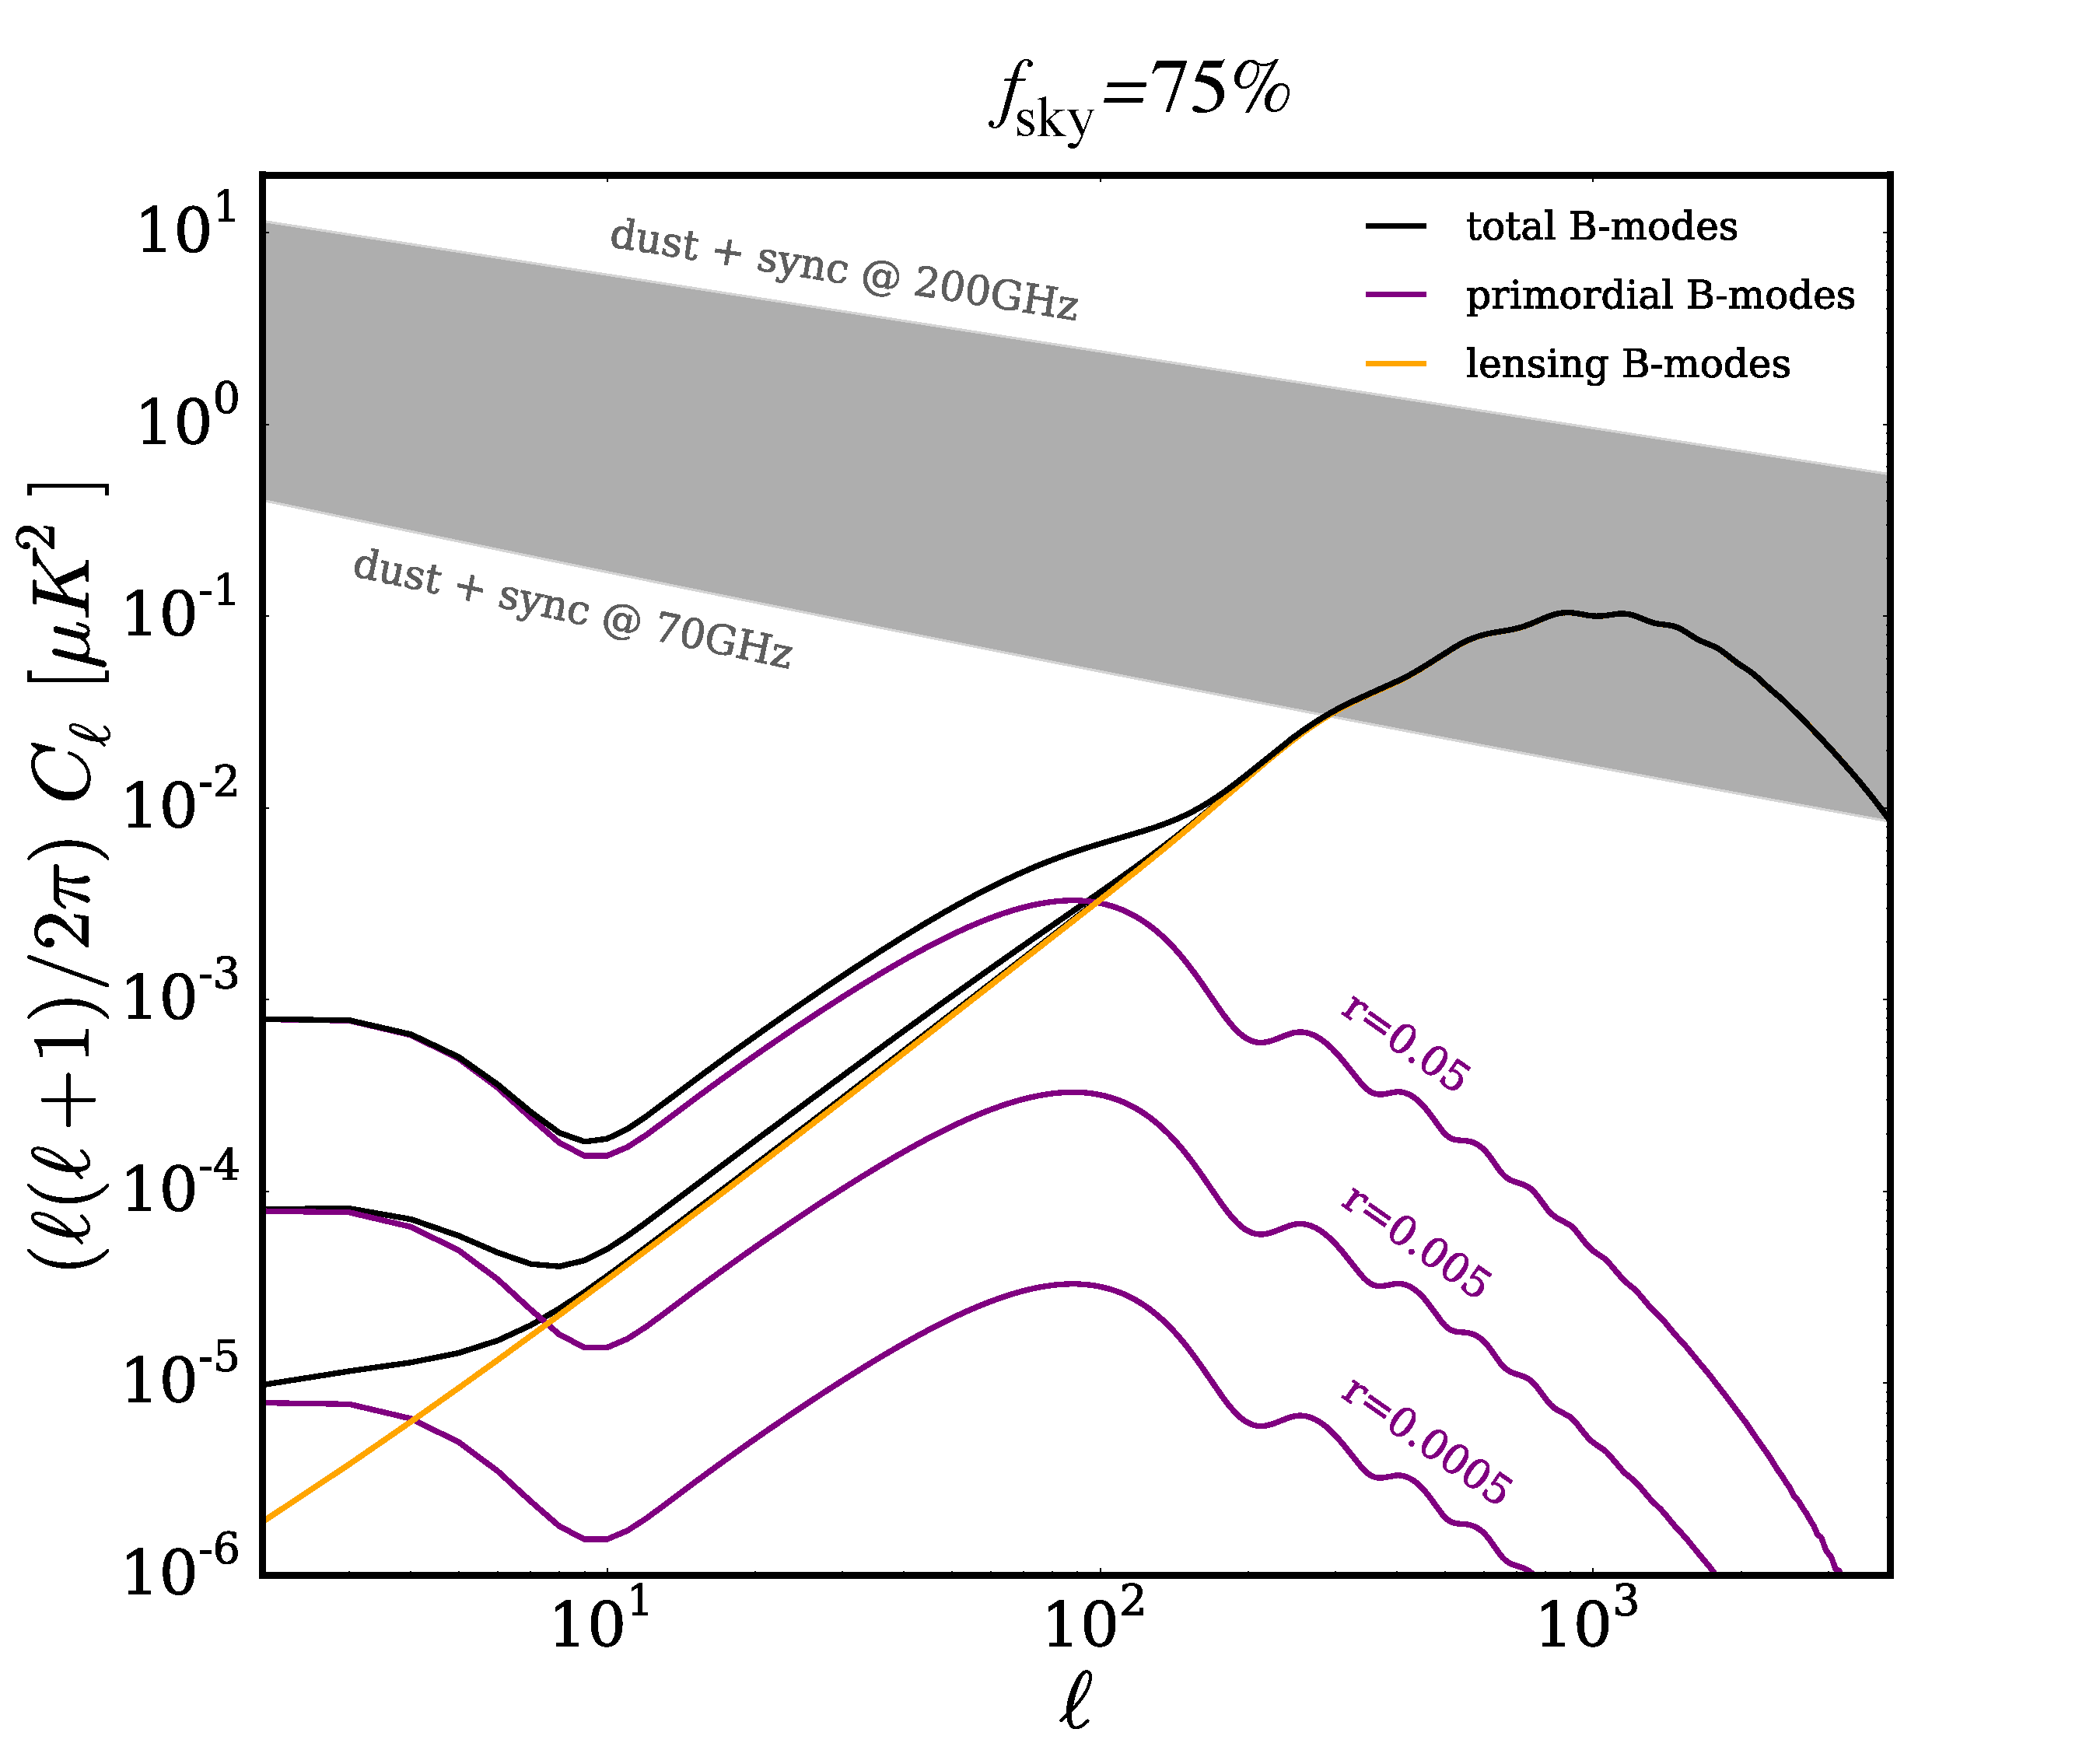
\includegraphics[width=3.12in]{Figures/clbb_freq.pdf}
\end{center}
\caption{}
\label{fig:frequency}
\end{figure}

\subsubsection{Systematic Effects}
\label{sec:systematics}
\begin{itemize}
\item Intensity-to-polarization leakage: Differential pointing,
  differential beams, gain errors, bandpass mismatch leakage 
\item Stability: Thermal drifts, space radiation environment
\item Straylight: polarized far-sidelobe pickup
\end{itemize}

% Raphael, Josquin, Aurelien, Charles


\vspace{-0.22in}


\subsection{The CMB Probe in Context}
\label{sec:spacemission}

\vspace{-0.05in}

\subsubsection{Current and Forthcoming Sub-Orbital Efforts}

The remarkable forthcoming scientific yield has motivated significant agency investments 
in current and future sub-orbital experiments which are designed to realize the full potential of this
unique probe of fundamental physics and astrophysics.    These experiments are designed 
to exploit the comparative advantages of the sub-orbital platforms, while providing the design heritage and 
experience necessary to maximize the probability of success of an orbital mission. 

For the ground-based efforts, these include combinations of {\it i)}
provision for large apertures and therefore high angular
resolution, {\it ii)} flexibility to rapidly deploy new technologies, and {\it iv)}
allowance for detector formats that are relatively unconstrained by
mass and power limitations.  To date, these have demonstrated low
noise measurements of small and intermediate angular scale $E$ and $B$ polarization 
structures over less than 2\% fractional areas of the sky. 


The balloon-borne missions {\it i)} extend the frequency reach of the ground based telescopes, 
{\it ii)} enable high fidelity measurements on larger angular scales than can be probed from the 
ground, and {\it iii)} grant access to an environment with similar requirements and constraints
as in orbit, providing heritage for future space missions as well as experience in dealing with the 
analysis of data that are representative of a space mission. In this way, the sub-orbital programs 
complement and multiply the scientific return of the proposed orbital mission, while reinforcing its 
technical preparedness.  

The 2010 Decadal Panel strongly recommended supporting sub-orbital efforts in preparation 
for a possible space mission to follow sub-orbital detections of inflationary gravity waves. 
As a result, the US has clear leadership in the field, both in terms of ground- and balloon-based 
experiments and results. 

This leadership will continue into the foreseeable future. In aggregate, funded, now-being-built 
`Stage 3' CMB experiments will deploy approximately 100,000 detectors on various sub-orbital 
experiments within the next 3-5 years. 
Ground-based experiments plan to extend measurements from few percent of the sky to 
few tens, although in a limited frequency range between 30 and 300~GHz. Balloon-borne 
payloads operating at even higher frequencies strive to cover even larger fractions.  

%As a result, noise levels will decrease, the foregrounds will progressively be better understood, 
%technologies will be tested, and we will have learned how to 

%Some funded ground-based efforts now being under construction or commissioning, are expected 
%to reach noise levels of ?? $\mu$ K arcmin over ??\% of the sky, in a limited frequency 
%range, between 90 and 280~GHz, and after ?? years of integration. 
%cite bicep/keck, spt
%Balloon-borne experiments plan to extend the measurement to much larger sky fractions, 
%up to 80\% in one case, and extend the frequency range to 600~GHz, 
%significant fractions of the full sky. 
%cite ACT
%Currently funded balloon borne
%experiments will add to this sensitive data at frequencies above 200
%GHz which will help characterize Galactic dust, while ground based
%experiments in Chile will add critical information at lower
%frequencies to constrain synchrotron emission.
%cite Spider Fraisse et al, Piper, Ebex, CLASS, ACT
%The Stage-4 experiments
%will extend these measurements to much larger areas, and to angular
%scales smaller than $5^\prime$, with benefits to the CMB Probe as
%described in Section \ref{sec:science}.

\vspace{-0.18in}

\subsubsection{Proposed Efforts: LiteBIRD, CORE, and CMB-S4} 

\vspace{-0.05in}

Japan, in collaboration with NASA, is now considering whether to proceed with LiteBIRD, a space mission 
designed to search for $B$ modes from inflation. The US Team has submitted its Phase A report to NASA; Phase A 
in Japan will conclude in about a year \comred{check}. LiteBIRD is a smaller, more focused
mission compared to the CMB Probe. It is an imager based on a 0.5~m aperture 
telescope. Therefore it has a resolution 4 times lower compared to the 2~m aperture of EPIC-IM. Its
reach in $\ell$ space is correspondingly 4 times lower making the science available at $\ell$'s above 
few hundred in both $E$ and $B$ modes unreachable. 
It has no spectroscopic capabilities and thus not sensitive to any of the spectral distortion science goals. 

For the Japanese space agency JAXA, LiteBIRD is meant to fit within the \$300M class of missions. 
Although there are uncertainties about comparing JAXA's cost calculations to NASA's, LiteBIRD's overall size 
and more limited science reach is commensurate with it being below, or just at the lower margin of the Probe's
cost window. 

A collaboration of scientists in Europe has just recently proposed CORE to ESA as part of the M5 round 
of space mission proposals. 
The team includes a number of US collaborators; the PI of this proposal is a member of 
CORE's Executive Board. CORE is a CMB polarization imager that is based on a 
1.2~m aperture telescope and thus intended to reach 2.5 times the resolution of LiteBIRD. ESA has 
capped the M5 proposals to EU550M, the equivalent of 
\$610M. Member countries are expected to contribute an additional $\sim$\$163M making the total 
cost close to \$773M. Selection of missions for Phase A studies is expected in fall 2017, and 
end of Phase A selection in fall 2019. 

The US CMB community has proposed, and the Particle Physics Project Prioritization Panel (P5) has recommended 
to the DOE, the establishment of a 4th generation CMB experiment called CMB-S4. This is an ambitious 
program to field approximately 5 times the number of detectors fielded by Stage 3 experiments. If and when funded, 
CMB-S4 will enable unprecedented sensitivity at frequency bands accessible from the ground, and 
with telescopes that enable high resolution. 

%A robust program of sub-orbital experimentation has proven a vital component in the success of all three generations of previous CMB orbital missions -- COBE, WMAP and {\it Planck}. Building on this heritage, the current (Stage-3) and planned (Stage-4) sub-orbital experiments are well poised to play a similar role for the CMB Probe, which will provide definitive measurements of the full sky from the largest angular scales to the $5^\prime$ scale of the beam.

\vspace{-0.18in}

\subsubsection{Why Study a CMB Probe?} 

\vspace{-0.05in}

Learning from the successes of COBE/FIRAS, COBE/DMR, WMAP, and \planck, a
CMB Probe is the single most suitable vehicle to deliver complete sky coverage 
and therefore information on the largest angular scales, 
comprehensive frequency coverage, and exquisite control of systematic effects. 
Some of the science goals described in Section~\ref{sec:science} 
are reachable only through mapping of the largest angular scales. No sub-orbital experiment 
has yet produced any polarization results on more than 2\% of the sky, let alone 
on scales requiring 70\% of the sky. The broad frequency coverage of the space 
mission is best suited to mitigate the foregrounds expected on a broad range of angular 
scales, including those important for removing the effects of B-modes from lensing. 
The mission will provide a single self-consistent and self-calibrated data set;  and it  
will provide legacy maps at many frequency bands that will become the basis for 
hundreds of new papers. 

If the Inflationary signal is detected by sub-orbital experiments
any time soon, a space mission to characterize the signal in full detail is equally compelling. 
The existence of ambitious sub-orbital programs is a complementary strength. How 
to make the best use of this complementarity is an explicit goal of our study; 
see Section{sec:management}.

\vspace{-0.18in}

\subsubsection{Does the CMB Probe Fit Within the Cost Window?} 

\vspace{-0.05in}

The total cost estimate for the EPIC-IM mission, as generated by JPL's Team X, was \$920M in 2009~\cite{}. 
The mission had a 1.4 m effective entrance aperture. When the mission was assessed
by the 2010 Decadal Panel, the independent cost estimate was \$1200M \comred{check}. The CORE mission, that had just been 
proposed to ESA and has an aperture of 1.2~m, was estimated by the proposing team to have a total cost \$773M. The cost
estimate for LiteBIRD, which has a 0.5~m aperture, is within the \$300M class. 

When NASA proposed to initiate studies for next-decade flagship missions that had a cost exceeding \$1B
there was consensus within the CMB community that a compelling CMB mission can be constructed for 
less than this amount.  The aperture size and science goals we are envisioning for the CMB mission 
are most akin to EPIC-IM and CORE and we therefore believe it fits within the Probe class. 

\vspace{-0.18in}

\subsubsection{This Study in the Context of Previous Mission Studies} 

\vspace{-0.05in}

The EPIC-IM summary paper and a report to the decadal panel from a NASA mission study, both from 2009, represent 
the US community's most recent view of the anticipated 
science reach and the path to implementation of a possible future US space mission. The landscape 
has changed since.  There is a need to present an updated view to the next decadal panel.  

Theoretical advances and progress in physics and astrophysics gave updated 
goals for the fidelity of measurements of $E$ and $B$ modes, including measurements of inflationary 
gravitational waves, the properties of light relics, and structure formation in the universe. A 
slew of sub-orbital experiments together with the \planck\ mission have 
transformed our view of the mm-wave polarized sky, highlighting the requirement on 
thorough understanding of the foregrounds. Advances in detector technologies, multiplexed readouts,
and optical components now enable a significantly more capable mission than the one envisioned
ten years ago. And the community has vastly more experience with designs of polarimeters and 
the control of their systematic uncertainties.  A new study, based on this accumulated information and 
experience, is timely; this is the study we are proposing here. 

The US LiteBIRD team has proposed participation in LiteBIRD and recently generated its Phase A 
report. The proposal and report were conducted by 
a subset of the community for the purpose of supporting a specific mission design, within specific 
cost caps, that match JAXA plans. 

Work on our proposal, and 
the subsequent mission study, represent a collaborative effort by all interested members of the 
CMB community, including US members of the LiteBIRD team. We have also reached out to our international partners 
and invited them to participate. The final report will present a consensus view of the US CMB community. 
This would be the proper input for the deliberations of the next US decadal panel. 





























\vspace{-0.22in}


\subsection{State of Technologies}
\label{sec:technologies}

\vspace{-0.05in}

\comred{2 pages. Discuss the technologies, their TRL, and what will be studied }
% Toki, Jeff

A fourth generation CMB satellite targeting a map sensitivity of $\sim1 \mu\mathrm{k-arcmin}$ will require, extremely sensitive detector arrays, tight control over systematics, and ability to reject polarized foregrounds as is described in Section 1.2.
Given the frequency dependance of synchrotron and dust foregrounds, this last requirement translates into the need for a large number of spectral bands covering the approximate frequency range from $\sim30$~GHz to $\sim800$~GHz.
Development of the CMB technologies needed to meet these requirements is actively being pursued by many groups who are also demonstrating these technologies on ground, balloon, and satellite platforms.   We describe the status and needs in the areas of telescopes, optics, detector coupling, detectors, and readout.

\paragraph{Telescopes:}  Carbon Fiber Reinforced Polymer (CFRP) mirrors are at TRL 9 as they have flown on the Planck sattelite. Their 1.9x1.5 m mirror weighted only 28 lbs and met all surface quality requirements. However, small deformations in the mirror caused by its structural supports had a measurable impact to the beam far-sidelobes that was not caputred by preflight measurements or the corresponding beam modeling.  Future CMB satellites will require improved pre-flight characterization of {\it polarized beam} at operating temperature augmented by improved simulation tools to meet even more systematics requirements.  Current ground and balloon born optical designs achieve large field of views (FOVs) with reflective and refractive designs; related designs and their implementation should studied in the context of a satellite mission as the sensitivity requirements lead to the need to maximize the size of the FOV while fitting within the tight mass and size constraints imposed by a space mission.  Given the heritage of past satellite missions it will be possible to develop a telescope design that meets the requirements for a future mission and uses high TRL components.

%State of the art CMB telescopes have apertures ranging from 0.3 to 10 meters in diameter with   designs including: on-axis refractive telescope (e.g. BICEP, SPIDER), crossed Dragone reflective telescope (e.g. QUIET, ABS) , and off-axis Gregorian reflective telescope (e.g. Planck, SPT, ACT, Simons Array, CLASS, EBEX). 

\paragraph{Optical Coupling:} 
The need for sensitivity drives the push for high efficiency optics; wide bandwidth to compliment mutichroic detector ; infrared filters to maximize cryogenic performance; and polarization modulators to suppress $1/f$ noise and mitigate instrument systematics.  The CMB field has made tremendous progress recently by drawing on advances in materials, processing techniques,  and developments in electrical engineering including meta-material research.  Single crystals such as silicon and sapphire are attractive since they offer extremely low dielectric losses and high indices of refraction to better manipulate light.  New coating techniques have been developed for silicon and sapphire that span 2:1 bandwidth (TRL 5+ for silicon) and can realize up to 5:1 bandwidth.  EBEX deployed broadband cryogenic polarization modulator with a superconducting bearing that covered 150~GHz band to 410~GHz band raising the modulators to TRL 5+ for space.  Meta-material metal-mesh optical filters were deployed with the Planck satellite and they are extensively used by ground based and balloon experiments making these TRL6 optical elements. It is necessary to develop a plan for a satellite mission that will cover $\sim30$~GHz to $\sim800$~GHz.  Two configurations could be considered: multiple optical paths with $<3:1$ bandwidth and a potentially simpler design with only two optical paths with  $\sim5:1$ bandwidth.   These studies include evaluating the design tradeoffs inherent to these approaches, developing the new coatings needed, and  evaluating the promise of hybrid approaches where filters and lenses are implemented in the same optical elements.  In addition, the cryogenic rotation mechanism should be demonstrated at the robustness (eg lifetime) needed for for a satellite mission.


\paragraph{Detector Coupling:} 
The focal-plane feed determines the shape and polarization properties of the pixel beams and therefore plays a strong role in controlling systematic errors. 
The feed design also can determine the total bandwidth and number of photometric bands of each pixel which is important for the efficient use of a telescope's focal plane area. 
CMB experiments developed broadband multi-chroic {\it detector} to increase optical throughput of a focal plane. 
Broadband feed captures signal over wide frequency range. 
Then on-chip superconducting filter partitions signal into multiple frequency bands prior to detection. 
Broadband detectors were realized with spline profiled horn and lenslet coupled antenna. 
Broadband horn detector deployed a pixel that covers 2.3:1 bandwidth with on going development for extending bandwidth to 6:1.
Broadband lenslet coupled antenna will deploy 3:1 bandwidth detector this year.
Lenslet coupled antenna demonstrated 5:1 bandwidth in laboratory. 
RF-techniques to partition broadband signals into multiple band are mature.
For a future CMB polarization satellite mission, broadband feed should be demonstrated at high frequency where alignment and line width for micro-fabrication becomes challenging. 
Detectors for CMB satellite mission were hand picked one by one for optimal performance.
Next generation of detector array will be fabricated on a silicon wafer. 
Micro-fabrication process should demonstrate high yield and uniformity across a wafer that can meet tight requirement of satellite mission.
Also detector test need to able to characterize detector beyond the level of systematic required by next generation CMB satellite experiment.

The Planck HFI deployed Neutron Transmutation Doped Germanium high-resistance bolometer at 100 milli-Kelvin to achieve photon noise limited detector performance.
A Transition Edge Sensor (TES) bolometer uses a steep transition of superconducting metal to improve linearity of the detector.
TES bolometers have been deployed on 100 milli-Kelvin and 250 milli-Kelvin platform. 
TES bolometers have been deployed across ground based and balloon CMB experiments spanning 40~GHz-410~GHz with detectors achieving NEPs of 20-50 aW/$\sqrt{\textrm{Hz}}$, nearly background limited at CMB frequencies. 
TES bolometers deployed at low optical frequencies ($\sim$40\,GHz) and balloon-borne payloads should realized even lower NEPs of $\sim$10\,aW/$\sqrt{\textrm{Hz}}$. 
Emerging detector technology for CMB experiment is kinetic-inductance detector (KIDs). 
The KIDs detector detects signal as change in kinetic inductance. 
KIDs detectors can be frequency multiplexed easily to $\sim1,000$ detectors.
Recently, on-sky demonstration at 150 GHz and 230 GHz was done with lumped element KID detector. 
Noise performance of KID detector at low frequency channels ($< 40$~GHz) need some improvement to be photon-noise limited. 
Currently there is no CMB polarizatin power spectrum data produced with KID detector.
Coupling between RF (100 GHz) signal to micro-wave KID (MKID) detector is in a development stage.
Planck detectors experienced unexpectedly high rate of cosmic ray events.
Data was successfully cleaned with analysis technique. 
Study of impact of cosmic rays on a detector is crucial for next CMB satellite mission.

Multiplexed readout is being used by CMB experiments to readout thousands of TES bolometers, and readout multiplexing is built into KID detector architecture. 
Voltage bias and low impedance of a TES bolometer facilitates multiplexing readout by Superconducting Quantum Interference Device (SQUID). 
Time domain multiplexing uses a SQUID at milli-Kelvin as a switch to rapidly cycle through bolometers. 
Highest achieved multiplexing factor is 64 channels.
Frequency domain multiplexing uses superconducting resonators to assign bolometers to different frequency channels.
Highest achieved multiplexing factor is 68 channels.
New readout scheme, such as microwave SQUID readout, is emerging to increase multiplexing factor for TES bolometer. 
MKID detector architecture has multiple resonators coming off from a transmission line. 
A resonator is both a detector and multiplexer. 
MKID demonstrated multiplexing factor that exceeds 1,000 channels. 
For next generation satellite experiment that will readout over thousands detectors require high multiplexing factor.
Multiplexing factor is directly related to readout complexity and power consumption.
Also the Planck mission experienced ADC non-linearity, thus extensive characterization of end to end readout archtecture should be performed pre-flight. 

A future CMB satellite mission offers exciting opportunity for millimeter wave polarization science. 
Experience from Planck mission will be studied to learn lessons for the future mission.
Development for CMB instrumentation is an active field with many institutions developing new technologies for ground based, balloon, and proposed satellite missions.
For a satellite instrumentation, there is a difficult trade off between desire to have high performance instrument and desire to keep cost manageable.
Many developments that is going on for ground based and balloon experiment have similar goal as satellite mission that collaborative development across all platform will be beneficial.



\vspace{-0.22in}


\subsection{Mission Study and Management Plan  }
\label{sec:management}

\vspace{-0.05in}


There are compelling science targets for an imager-based and for 
a spectrometer-based CMB Probe. Our study will investigate the science and technical trade-offs 
for both of these options, and for a combined mission. 

The study itself is open for the entire CMB community and already includes more than 40 scientists representing 
hundreds of years of experience with CMB theory, data analysis, and measurements on all platforms including satellite missions
that have already flown (WMAP, and \planck ) and the two proposed (LiteBIRD and CORE). 
Figure~\ref{fig:management} shows the management structure of the collaboration. The PI Hanany, who has more 
than 20 years of CMB ballooning experience, co-led MAXIMA and Archeops, was the PI of MAXIPOL and EBEX, and 
is a member of the CORE steering group, will have ultimate responsibility for the study. He 
is advised by a Steering Committee -- Bennett (Johns Hopkins), Dodelson (Chicago), and Page (Princeton) -- 
and assisted by a business office at the University 
of Minnesota.  An Executive Committee (EC) is in charge of the daily operation of the collaboration. The PI and each member of the 
EC also have responsibility for a particular study working group (WG), as outlined in the Figure. Significant overlap and feedback is 
expected among the WGs. 

%and as outlined in more detail below? 
%NASA/JPL, lead by CoI Lawrence (Chief Scientist 
%at JPL and US \planck\ team lead), will assist with mission design. The PI will lead the study of the Imager and will interface with 
%the JPL team. Al Kogut (PI of the Explorer-proposed PIXIE) will lead the spectrometer study. Knox and Flauger will lead the theory and 
%foregrounds aspects of the study; McMahon and Lee (PI of the US LiteBIRD team) will lead the study of relevant technologies.  

\begin{figure}[ht!]
\hspace{-0.1in}
\parbox{3.5in}{\centerline {
\includegraphics[width=3.5in]{../OrgChart_Names} } }
\hspace{0.05in}
%\end{center}
\parbox{2.5in}{
\caption{ \small \setlength{\baselineskip}{0.95\baselineskip}
Management structure of the CMB Probe. An Executive Committee led by the PI manages the work of the entire team. 
Membership in the team is open to all members of the CMB community. Working groups, led by members of the executive 
committee, investigate and develop aspects of the mission. 
\label{fig:management} } }
\vspace{-0.1in}
\end{figure}


The study will be carried out through intra- and inter-WG teleconferences; mission design teleconference with JPL engineers; 
mission design meetings at JPL; and a community workshop that is described in more detail below under the `Space / Sub-Orbital 
Synergy' WG. We now describe the planned work for each of the WG. 

$\bullet$ {\bf Theory (Knox)} \hspace{0.1in} This WG will survey, summarize, and prioritize the set of 
science goals for the Probe.  Given input on target frequency bands and instrument noise levels the group will 
generate forecasts for the impact of the Probe's products and their ultimate 
significance for physics and astrophysics.

$\bullet$ {\bf Mission (Hanany) and connection with JPL (Lawrence)} \hspace{0.1in} The Mission WG is responsible 
for defining the overall mission 
architecture including telescope implementation, cooling, telemetry, mass, power, and cost. The WG will work closely 
with the JPL lead scientist (Lawrence) and JPL mission engineers. 

$\bullet$ {\bf Imager (Hanany) and Spectrometer (Kogut)} \hspace{0.1in} The imager and spectrometer WGs will 
translate the science goals to 
mission requirements and to a set of optional designs. The designs will include telescopes of various configurations, 
focal planes with several candidate detector technologies and readout schemes. These groups will similarly consider 
the options for spectrometers.  Both groups will work closely 
with the mission WG and with the JPL team to assess the relative merits 
of the optional designs, which will include an imager-only and spectrometer-only options, as well as a combined
instrument.  

$\bullet$ {\bf Space / Sub-Orbital Synergy (Jones, Devlin)} \hspace{0.1in} By the time the \ac{CMB} probe is likely to fly,
significant advances are expected to be made on the ground. This is true regardless of the state of the proposed CMB-S4
effort, and even more so should funding for S4 becomes available soon. This working group will assess and recommend the 
most appropriate design parameters such that the data sets from the Probe and sub-orbital measurements complement each other. 
Pertinent questions include: to what extent should the aperture size of the Imaging Probe rely on delensing capabilities provided by 
high resolution measurements from the ground? What is the optimal resolution of a space based mission from the point 
of view of providing foreground subtraction capabilities to sub-orbital missions? What is an optimal overlap in $\ell$-space
coverage? Does the design of a spectrometer depend on the specifics of data available from sub-orbital measurements? 

We are planning a community workshop to address these question, including forming a community consensus on the 
question of the need for a space mission if CMB-S4 is funded. 

$\bullet$ {\bf Complementarity with Other Data Sets (Pryke)} \hspace{0.1in}
The full sky nature, the broad frequency coverage, and the high sensitivity of the CMB-Probe will generate legacy 
data set surpassing that of \planck 's. This working group will survey the possible cross-correlations with astrophysical 
data available at other wavelengths. It will assess whether such cross-correlations can benefit by preferring 
some mission parameter values over others. Examples include adjusting the resolution, and frequency coverage. 
The group will also survey possible sources of systematic uncertainties and how these can be addressed during mission 
design, implementation, and data analysis. 

$\bullet$ {\bf Systematics (Crill)} \hspace{0.1in}

$\bullet$ {\bf Foregrounds (Flauger) } \hspace{0.1in}

One of the key ingredients in the design of a CMB experiment is the frequency coverage required to achieve the science goals. Consequently, optimizing frequency coverage in light of the new information from $Planck$ and its limitations will be one of key task of the study proposed here. 

%OVERVIEW of PLAN
To achieve these goals we plan a careful investigation of the effect on the measurements of r and $\tau$ of the presence of foreground residuals in the CMB maps (after foreground separation and/or cleaning) including, for example, the properties of the polarized thermal dust emission, specifically the spatial variation of its spectral index (hinted at by the observed decorrelation of the dust between 217 GHz and 353GHz Planck channels \ref{Planck2015-X;Planck2015-L;Planck2015-XXIX;Boulanger2016}), the breakdown of the modified black body spectrum model, and decorrelation between frequencies. 

These aspects will be explored with the help of physically motivated models of the foregrounds (\ref{Bruce+Fraisse2009,Hensley et al in preparation}) informed by existing data along with simulations based on these models. To incorporate instrument systematics due to beams, bandpass mismatches, correlated noise, etc., time domain based simulations will be required.

%INSTRUMENTAL PARAMETERS:
To devise the optimal instrumental/observational concept/design we will probe several configurations by varying critical instrumental parameters such as: the frequency coverage, the number of frequency channels, inter-band separation (limited by the typical instrumental bandwidths), the noise or sensitivity of each frequency channel, and angular resolution. 

%FG MODELLING:
Given that the B-mode signal is very weak, and much fainter than galactic foreground emission, even slight inacuracies in the characterization of the foregrounds will potentially impact the detectability of the B-mode signal. Therefore it is crucial to consider a large frequency coverage to properly gather the nature of the foregrounds as well as 'realistic' models that capture intrinsic complexities of these diffuse polarized foregrounds.
Therefore we will consider physically motivated dust models (beyond the modified blackbody spectrum approximation) currently in development. 
For these models the absorption cross-section in Intensity and Polarization are estimated self-consistently for grains of different sizes, shapes, and compositions as a function of frequency. These physical dust models will be used along with models implemented in the Planck Sky Model, PSM \ref{}, and/or  Python Sky model, PySm \ref{}, 


%TECHNIQUES:
To forecast the performance of a given instrumental design we will resort, for a quick diagnosis, to traditional techniques such as Fisher codes, both spectra and map based, that account for the presence of foregrounds assuming some best fit model of both the CMB and Foregrounds (akin to those used for the CMB-S4 science book \ref{}, eg CMB4cast (http://portal.nersc.gov/project/mp107/index.html)). 

%SIMULATIONS
For a more in depth analysis, that can also probe biases in the parameters, we will simulate maps of the CMB and Foreground emission at each frequency with CAMB and PSM (or PYSM) packages respectively and HEALpix modules \ref{}. Noise simulations will then be added to the signal maps.
While white noise or anisotropic noise are straightforwardly simulated directly on map domain, 1/f or correlated noise requires simulating time ordered data according to a noise prescription or generator (eg akin to LevelS \ref{} used in Planck). The convolution of the simulated maps with the Gaussian beams can be performed straightforwardly with HEALpix modules, while the convolution with more realistic beams is harder but can be performed with approaches such as FEBeCOP \ref{}, developed for Planck data analysis. To apply the latter an optical beam and scanning strategy needs to be specified and adopted by the software.

The next step is to clean the frequency maps from foregrounds and generate the 'clean' CMB map, using techniques such as Commander, SMICA, SEVEM and possibly NILC \ref{Planck2015-IX}. This is followed by estimation of auto and cross-correlation angular power spectra of the maps using say Master based \ref{}  or XFaster \ref{} based techniques and propagated to parameter estimation using CosmoMC or Multinest sampling.
Along with this standard procedure we will also apply a novel technique based on direct Bayesian MCMC inference of cosmological parameters in the presence of foregrounds, without resorting to Likelihood approximations (an extension of the method presented in  \ref{Jewelletal2016}). 
The latter will be integrated with Commander, allowing to bypass the angular power spectrum estimation as it samples Cosmological and Foregrounds parameters directly from the simulated maps. As in this approach the foreground parameter fits (including the spectral index) is performed pixel by pixel, the spatial variation of the spectral index is naturally accounted for. 

%As mentioned earlier 1/f or correlated noise requires simulating time ordered data. To analyse the resulting maps another ingredient is needed, the pixel-to-pixel noise correlation matrix. For a large number of pixels the estimation of this matrix is computationally intensive. As 1/f and correlated noise leaves mostly in the large angular scales and we resort to studying these effects on low resolution maps (reducing computational costs), hybridized with higher resolution maps for the white noise component. 

It should be stressed that to fully assess the performance of a given instrument design, in view of both foreground residuals and the presence of systematics, realistic simulations are essential. These include time domain based simulations which can be generated using HPC4CMB ((https://github.com/hpc4cmb)) based on TOAST 
%(data framework, including on-the-fly simulation capabilities with full detector beam, bandpass and noise properties)), 
and a destriper based map-making algorithm such as libMADAM. 


%FOM
Finally to quantify performance we will need to define a figure of merit, FOM. Examples of possible FOM, are: the effective noise in the I,Q,U maps after foreground cleaning (effectively quantifying the noise degradation due to the presence of residual foregrounds); uncertainty and biases in the parameters; the evidence of the best fit model for each instrumental design (used as a qualifier of the instrumental design itself), etc.


\comred{GR:This is a first version of the plan - still needs editing} 
 




$\bullet$ {\bf Technology (Lee, McMahon)} \hspace{0.1in}


Sub-orbital measurements are complementary to those made aboard a space probe. By the time the \ac{CMB} probe is likely to fly significant advances are expected to be made on the ground. 



\newpage

\bibliography{mybib,Ref_SD}

\newpage

\section{Curriculum Vitae}
\label{sec:cv}

\newpage
\addtocounter{page}{8}
\section{Summary of Work Effort}
\label{sec:workeffort}

\section{Current and Pending Support}
\label{sec:current_and_pending}

\newpage
\addtocounter{page}{13}
\section{Letters of Support}
\label{sec:lettersofsupport}

\newpage
\addtocounter{page}{3}


\section{Budget Justification}
\label{sec:budget}

\subsection{General}
\label{sec:budget_general}

The majority of funding is allocated to these categories of expenses: summer salary, primarily for the PI who will 
coordinate the entire effort; travel of team members to JPL to participate in mission design sessions; 
the community workshop that will discuss the complementarity between a future space mission and sub-orbital efforts. 

\subsection{Funded Team Members}

The PI Shaul Hanany requests 4 weeks of summer salary in year 1 and 3 weeks in year 2.  We are 
also requesting 2 weeks of summer salary to support Knox, the CoI organizing the theory effort. 

Support for an administrative assistant is required due to the demand on regular staff that usually 
accompanies putting on a workshop.  This effort is above their normal departmental duties.  The assistant 
will help organize the workshop and develop a website, process registrations, secure accommodations 
and make other travel arrangements for workshop attendees, work outside their regular work hours attending 
the meeting and troubleshooting, and will have to process numerous reimbursements.  The assistant will also 
assist with the community organization tasks during the rest of the year.  

\subsection{Travel}

Travel funds are requested for the PI and four others to go to Pasadena, CA to collaborate with 
JPL�s Advanced Projects Design Team (Team X).  There will be 2 trips in each budget period.  One longer trip 
of 3 days/2nights and one shorter one of 2 days/1 night.  Both trips are based on airfare of \$500, 
lodging of \$150/night, and meals of \$64/day with 75\% on the first and last day and about \$250 for 
ground transportation and other incidentals.  This comes to \$11,000 per budget period 
(5 person-trips at \$1,200 + 5 person-trips at \$1,000).

Also included, is travel for the PI to the AAS 2018 Conference in Budget Period 2, which per 
the NRA, is where a presentation of findings will be most likely be made.  The cost of this trip is \$1,700 and is 
based on airfare to Washington, DC of \$500, \$226/night hotel  x 3, \$69/day for meals using 75\% for the first 
and last day), and then \$217 for ground transportation and incidentals.

All travel is based on the published GSA rates at the time of this proposal.

\subsection{Workshop}

A research collaboration workshop will be held in Budget Period 1, most likely in the summer of 2017.  
It will be attended by approximately 150 people, both domestic and foreign.  The cost of \$30,000 is based on 
partial travel support and local lodging for about 25 attendees at \$1,000 per person = \$25,000.  In addition, 
there will be venue rental costs and provisions for the meetings; breakfast foods, afternoon snacks and 
beverages for coffee breaks (\$5,000).  

\subsection{Publications}

We are planning to publish the results of our study. Page charges of \$1,100 are included in both budget periods.  
A likely journal is the Astrophysics Journal.  Page charges are based on publishing a a 10-page article each year.  
The current rate is \$110 for an electronic submission.  

\subsection{Communication Costs:}
This project will required several weekly telecons.  The cost budgeted is based on a monthly cost of about \$65
based on experience with other projects.




\newpage
%\addtocounter{page}{9}

\section{Budget Sheets}

\end{document}

%\begin{table}[h] %%[h]
%\begin{center}
%\begin{tabular}{|c|c|c|c|c|c|} \hline 
%\multicolumn{6}{|c|}{Summary of Personnel and Work Efforts, (Page 1 of 2)}              \\ \hline
%Personnel & \multicolumn{5}{c|}{Budgeted Effort/Year (months)}  \\ \cline{2-6}
%                 & Year 1  & Year 2 & Year 3 & Year 4   & Year 5   \\ \hline
%\multicolumn{6}{|c|}{\textcolor{blue}{University of Minnesota } }              \\ \hline
%Hanany,  PI              & 1/1  & 1/1 & 1/1 & 1/1 & 1/1  \\ \hline
%\multicolumn{6}{|c|}{\textcolor{blue}{Cal Tech } } \\ \hline
%Jamie Bock, Co-I           &  0.25  & 0.25 & 0.25 & 0.25 & 0.25  \\ \hline
%\multicolumn{6}{|c|}{\textcolor{blue}{Princeton} }  \\ \hline
%Lyman Page, Co-I           & 1/1  & 1/1  & 1/1  & 1/1   & 1/1  \\ \hline
%\multicolumn{6}{|c|}{\textcolor{blue}{Goddard Space Flight Center } }  \\ \hline
%Al Kogut, Co-I               & 0.75 & 0.75 & 0.75 & 0.75  & 0.75   \\ \hline
%\multicolumn{6}{|l|}{ $^{1}$ PDR = Post-Doctoral Researcher; } \\ 
%\multicolumn{6}{|l|}{ $^{2}$ GSRA = Graduate Student Research Assistant;  } \\ \hline
%\end{tabular}
%\end{center}
%\vspace{-0.2in}
%\caption{ Personnel, time in months on the project funded by NASA/time in months on the project not funded by NASA, and their role.  When 
%only one time value appears it is time funded by NASA.  {\bf Continued on next page}.
%\label{tab:personnel} }
%\end{table}

%\newpage

%\begin{table}[h] %%[h]
%\begin{center}
%\begin{tabular}{|c|c|c|c|c|c|} \hline 
%\multicolumn{6}{|c|}{Summary of Personnel and Work Efforts, (Page 2 of 2)}              \\ \hline
%Personnel & \multicolumn{5}{c|}{Effort/Year (Months)}  \\ \cline{2-6}
%                 & Year 1  & Year 2 & Year 3 & Year 4    &  Year 5    \\ \hline
%\multicolumn{6}{|c|}{\textcolor{blue}{Johns Hopkins} }  \\ \hline
%Chuck Bennett, Co-I               & 0.5 & 0.5 & 0.5 & 0.5  & 0.5   \\ \hline
%\multicolumn{6}{|c|}{\textcolor{blue}{NIST } }  \\ \hline
%Hubmayr, Co-I    &  0/0.25 & 0/0.25 & 0/0.25 & 0 &  0 \\ \hline
%\multicolumn{6}{|c|}{\textcolor{blue}{Lawrence Berkeley National Lab} }  \\ \hline
%Borrill, Collaborator   &  0  &  0  & 0 & 0 & 0  \\ \hline
%\end{tabular}
%\end{center}
%\vspace{-0.1in}
%\end{table}

%\newpage
%\addtocounter{page}{8}


%%%%%%%%%%%%%%%%%%%%%%%%%%%%%%%%%%%%%%%%%%%%%


%\begin{figure}%[thbp!]
%\hspace{-0.35in}
%\parbox{2.2in}{ \centerline {
%\includegraphics[height=2.2in] {Figures/GondolaZoom}} }
%\hspace{0.in}
%\parbox{2.2in}{ \centerline {
%\includegraphics[height=2.3in] {Figures/ebexmodel2016}} }
%\hspace{0.in}
%\parbox{2.2in}{ \centerline {
%\includegraphics[height = 2.in]{Figures/RayTrace_current}}}
%\vspace{-0.15in}
%\caption{ \small \setlength{\baselineskip}{0.90\baselineskip}
%	{\bf Left Panel}: The \ebextw\ experiment on the launch pad in Antarctica prior to its long duration flight. 
%	{\bf Middle and Right Panels:} A solid model with major gondola
%	elements and overview of the optical system for \ebexsk ; see also Fig.~\ref{fig:ebexskfocalplane}. 
%	Relative to \ebextw\ the sun-shade structure will change and the solar panels 
%	will be mounted on the side to allow observations of the BICEP2 region.
%	\label{fig:ebexpreflight} }   
%\vspace{-0.1in}
%\end{figure}

%\begin{table} 
%\begin{center} 
%\begin{tabular}{|c|c|c|c|c|c|c|} \hline \hline
%Task        & Gondola    & \multicolumn{2}{c|} {Optics + Receiver}     & Detectors & \multicolumn{2}{c|}{ Readout}  \\ 
%\hline
%Task Leader & {\it Johnson + Tucker$^{1}$ } & \multicolumn{2}{c|} {\it Hanany+McMahon} & {\it Lee} & \multicolumn{2}{c|}{\it Dobbs} \\
%\hline
%Institution & {\it Columbia + Brown$^{1}$ } & \multicolumn{2}{c|}{\it UMN+Michigan}  & {\it UCB} & \multicolumn{2}{c|}{\it McGill}   \\ 
%\hline \hline 

%Task   &  \multicolumn{2}{c|}{Attitude Control }   &  IR Filters & Foregrounds & \multicolumn{2}{c|}{Theory + Analysis}  \\ 
%\hline
%Task Leader & \multicolumn{2}{c|}{\it Miller  } & {\it Ade + Tucker} & {\it Baccigalupi} &\multicolumn{2}{c|}{Stompor, Jaffe} \\  \hline
%Institution & \multicolumn{2}{c|}{\it Columbia } & {\it Cardiff} & {\it SISSA} &\multicolumn{2}{c|}{APC - Paris, Imperial }   \\  \hline \hline 
%\multicolumn{7}{|l|}{$^{1}$ {\footnotesize Brown contributes specific separable elements to the gondola hardware} } \\  \hline \hline 
%\end{tabular}
%\vspace{-0.1in}
%\caption{\footnotesize \setlength{\baselineskip}{0.95\baselineskip}
%	Tasks and task leaders and institutions for the EBEX project. }
%\label{tab:tasks}
%\end{center}
%\vspace{-0.25in}
%\end{table}


%\begin{table}[h]
%%\hspace{-0.2in}
%\begin{center}
%\begin{tabular}{cccccc} 
%\hline \hline
%Pixel & Center Frequency & FWHM & NET/detector & Detectors & Array NET \\
% Type & (GHz) & (arcmin) &   (\microkrtsec)$^{a}$  & (\#) & (\microkrtsec)$^{a}$  \\ 
%   \hline
%          \multirow{2}{*}{Low Frequency}    & 150/180$^{b}$ & 7.2/6.0  & 142/148  & 2316/2316  & 2.95/3.08 \\
%          \multirow{2}{*}{(2316 pixels)}    & 250 & 4.4  & 248  & 3202  & 4.38 \\  
%                                            & 320 & 3.6  & 498  & 2648  & 9.68 \\  
%   \hline
%           \multirow{2}{*}{High Frequency}  & 220 & 4.9  & 219  & 3360  & 3.78 \\    
%           \multirow{2}{*}{(1680 pixels)}   & 280 & 3.9  & 361  & 3360  & 6.23 \\ 
%                                            & 360  & 3.2  & 956 & 3360  & 16.5 \\ 
%   \hline
%          Total                             &    &      &       & 20562 &      \\
%   \hline
%\multicolumn{4}{l}{$^{a}$ {\small Thermodynamic units; multiply by $\sqrt{2}$ for Stokes $Q,U$}} \\
%\multicolumn{6}{l}{$^{b}$ {\small Half of the pixels are with 150~GHz, the other half with 180~GHz (see Section~\ref{sec:detectors}) }} \\ \hline \hline
%\end{tabular}
%\end{center}
%\vspace{-0.2in}
%\caption{\small \setlength{\baselineskip}{0.90\baselineskip}
%	Specifications of the \ebexsk\ focal plane multi-chroic pixels and detectors.  The calculation of incident optical power 
%	assumes a bandwidth $\Delta \nu / \nu = 23\%$ and includes all known
%	contributions: the CMB, atmosphere, warm mirror, warm vacuum window, filters, cold lenses, 
%	and cold half-wave plate.  Thermal noise is calculated assuming that the
%	thermal conductance of the TES is optimized for 2.5 times the 
%	absorbed optical power. TES absorption efficiencies are 
%	assumed to be 0.7, 0.7, 0.65, 0.6, 0.6, 0.55 and 0.50 for 150~GHz and higher bands, respectively. 
%	See Section~\ref{sec:detectors} for more details on the focal plane layout.}
%\label{tab:band_sens}
%\vspace{-0.1in}
%\end{table}
%\vspace{-0.1in}
%\noindent\rule{6.5in}{0.4pt}
%%\vspace{-0.15in}


